\chapter{Stützstellen auf dem Einheitskreis}
% FIXME: Bad section title.
\section{Numerische Vorbetrachungen}

Im Folgenden zeigen wir, dass die Kondition einer Vandermonde-Matrix bezüglich
gewöhnlicher Normen\footnote{}%TODO
invariant unter Rotation und Spiegelung der Knoten ist.

%TODO: Was bringt das?

\begin{lemma}
    \label{lemma:vandermonde_rotation_invariance}
    Die Kondition der Vandermonde-Matrix bezüglich der Zeilensummennorm ist
    invariant unter Multiplikation der Knoten mit einer komplexen Zahl
    $\alpha = e^{i\varphi} \in \C$, $\varphi \in \R$.
\end{lemma}

\begin{proof}
    Sei $z = (z_0, \dots, z_{n-1}) \in \Cn$.
    Wegen $\abs{e^{i\varphi}} = 1$ für alle $\varphi \in \R$ gilt
    \[
        \begin{split}
            \norm{\Vand{\alpha z}}_\infty
            &= \max_{k=0, \dots, n-1} \sum_{j=0}^{n-1} \abs{\left(e^{i\varphi} z_j\right)^k}
            = \max_{k=0, \dots, n-1} \sum_{j=0}^{n-1} \abs{e^{ik\varphi}} \abs{z_j^k}\\
            &= \max_{k=0, \dots, n-1} \sum_{j=0}^{n-1} \abs{z_j^k}
            = \norm{\Vand{z}}_\infty.
        \end{split}
    \]

    \noindent Für die Zeilensummennorm der inversen Vandermonde-Matrix erinnern wir uns an Gleichung
    (\ref{eq:inverse_vandermonde_const_multiplication})
    aus Lemma \ref{lemma:inverse_vandermonde_const_multiplication}:
    $\tilde{u}_{jr} = u_{jr} \alpha^{-n+r+1}$.
    Damit ist sofort ersichtlich
    \[
        \begin{split}
            \norm{\Vand{\alpha z}^{-1}}_\infty
            &= \max_{j=0, \dots, n-1} \sum_{r=0}^{n-1} \abs{\tilde{u}_{jr}}
            = \max_{j=0, \dots, n-1} \sum_{r=0}^{n-1} \abs{u_{jr}} \abs{\alpha^{-n+r+1}}\\
            &= \max_{j=0, \dots, n-1} \sum_{r=0}^{n-1} \abs{u_{jr}}
            = \norm{\Vand{\alpha}^{-1}}_\infty.
        \end{split}
    \]

    \noindent Wie behauptet, folgt insgesamt
    \[
        \begin{split}
            \cond{\Vand{\alpha z}}_\infty
            &= \norm{\Vand{\alpha z}}_\infty \norm{\Vand{\alpha z}^{-1}}_\infty\\
            &= \norm{\Vand{z}}_\infty \norm{\Vand{z}^{-1}}_\infty
            = \cond{\Vand{z}}_\infty.
        \end{split}
    \]

\end{proof}

\begin{lemma}
    Sei $\emptynorm$ eine Matrix-Norm die invariant unter Multiplikation mit unitären
    Matrizen ist, d.h. für jede Matrix $A \in \C^{n\times n}$ und jede
    unitäre Matrix $U \in \C^{n\times n}$ gilt $\norm{UA} = \norm{AU} = \norm{A}$.
    Weiter seien ein Vektor $z = (z_0, \dots, z_{n-1}) \in \Cn$ und eine
    komplexe Zahl $\alpha \in \C$ mit Betrag $\abs{\alpha} = 1$ gegeben.
    Dann gilt für die Kondition bezüglich der Norm $\emptynorm$:
    \[
        \cond{\Vand{\alpha z}} = \cond{\Vand{z}},
    \]
    d.h. die Kondition der Vandermonde-Matrix ist in diesem Fall invariant
    unter Multiplikation der Knoten mit einer komplexen Zahl $\alpha$ vom
    Betrag $\abs{\alpha} = 1$.
\end{lemma}

\begin{proof}
    Wir setzen
    \[
        V = (v_{kj})_{k,j=0}^{n-1} \defeq \Vand{z}, \;
        \tilde{V} = (\tilde{v}_{kj})_{k,j=0}^{n-1} \defeq \Vand{\alpha z}
    \]
    und zeigen $\norm{\tilde{V}} = \norm{V}$ und
    $\norm{\tilde{V}^{-1}} = \norm{V^{-1}}$.

    \noindent Es gilt für $j,k = 0,\dots,n-1$:
    \[
        \tilde{v}_{kj} = (\alpha z_j)^k = \alpha^k z_j^k = \alpha^k v_{kj},
    \]
    d.h. wir können
    \[
        \tilde{V} = \diag{\alpha^0, \dots, \alpha^{n-1}} \cdot V
    \]
    schreiben.

    \noindent Für die inverse Vandermonde-Matrix hatten wir bereits in
    Lemma (\ref{lemma:inverse_vandermonde_const_multiplication})
    gesehen, dass $ \tilde{V}^{-1} = \alpha^{-n+1} \cdot V^{-1} \cdot \diag{\alpha^{0}, \dots, \alpha^{n-1}} $ gilt.

    \noindent Weiter können wir uns leicht davon überzeugen, dass
    $\diag{\alpha^0, \dots, \alpha^{n-1}}$
    für $\alpha = e^{i\varphi}$, $\varphi \in \R$
    eine unitäre Matrix ist, denn es gilt:
    \[
        \begin{split}
               \diag{\alpha^0, \dots, \alpha^{n-1}} \cdot \diag{\alpha^0, \dots, \alpha^{n-1}}^{H}
            &= \diag{\alpha^0, \dots, \alpha^{n-1}} \cdot \overline{\diag{\alpha^0, \dots, \alpha^{n-1}}}\\
            &= \diag{1, e^{i\varphi} \cdot e^{-i\varphi}, \dots, e^{i\varphi (n-1)} \cdot e^{-i \varphi (-n+1)}}\\
            &= \diag{1, \dots, 1}.
        \end{split}
    \]

    \noindent Damit erhalten wir
    \[
        \begin{split}
            \cond{\Vand{\alpha z}}
            = \cond{\tilde{V}}
            &= \norm{\tilde{V}} \norm{\tilde{V}^{-1}}\\
            &= \norm{\diag{\alpha^0, \dots, \alpha^{n-1}} \cdot V} \norm{\alpha^{-n+1} \cdot V^{-1} \cdot \diag{\alpha^0, \dots, \alpha^{n-1}}}\\
            &= \norm{V} \norm{V^{-1}}
            = \cond{V} = \cond{\Vand{z}}.
        \end{split}
    \]
\end{proof}

\section{Stützstellen auf dem Gitter der \boldmath{$N$}-ten Einheitswurzeln}
Seien $M, N \in \N$ mit $M < N$.
In diesem Abschnitt untersuchen wir Anordnungen von $M$ Knoten auf dem Gitter
der $N$-ten Einheitswurzeln und die Kondition der daraus resultierenden
Vandermonde-Matrizen.
Da in unserem Fall
\footnote{Wir betrachten nur die Zeilensummennorm und unitär invariante Normen bzw. die Kondition bzgl. dieser Normen.}
die Kondition einer Vandermonde-Matrix invariant unter
Permutation der Spalten ist, kommt es nicht auf die Reihenfolge der Knoten an.
Wir betrachten also genau die $M$-elementigen Teilmengen von
$\{ \exp( \frac{2 \pi i k}{N} ) \; | \; k \leq N \}$.
Diese können wir bekanntlich auf eindeutige Weise mit $M$-elementigen
Teilmengen von $ \Z / N\Z$ identifizieren, indem wir die Abbildung
\[
    \left\{ \exp( \frac{2 \pi i k_j}{N} ) \; | \; j = 1,\dots, M \right\} \mapsto \left\{ k_j \in \Z/N\Z \; | \; j = 1, \dots, M \right\}
\]
verwenden.
Diese motiviert die folgende Definition:

\begin{mydef}[Knotenset]
    Wir bezeichnen eine $M$-elementige Teilmenge von $\Z/N\Z$
    als \emph{Knotenset der Ordnung $(M,N)$}.\\
    Wir identifizieren ein Knotenset
    $S = \{k_1, \dots, k_m\} \subset \Z/N\Z$
    mit einer Menge von $M$ verschiedenen $N$-ten Einheitswurzeln durch
    \[
        S \mapsto e(S, N) \defeq \left\{ e^{\frac{2 \pi i k_1}{N}}, \dots, e^{\frac{2 \pi i k_n}{N}} \right\}.
    \]
    Da die Kondition einer Vandermonde-Matrix invariant unter Permutationen der
    Knoten ist, definieren wir weiter die Kondition eines Knotensets $S$ durch
    \[
        \cond{S} \defeq \cond{\Vand{ e^{\frac{2 \pi i k_1}{N}}, \dots, e^{\frac{2 \pi i k_n}{N}} }}.
    \]
\end{mydef}

% SECTION:OUTLIER
\section{Vandermonde-Matrizen aus \boldmath{$(n\!-\!1)$} Einheitswurzeln und einem Ausreißer}

Die Kondition bezüglich der Zeilensummennorm der Vandermonde-Matrix zu den $n$
Knoten der $n$-ten Einheitswurzeln beträgt $n$.

Im Folgenden untersuchen wir die Kondition einer Vandermonde-Matrix, bei der
einer der Knoten von seiner ursprünglichen Position als $n$-te Einheitswurzel
um einen Winkel $\delta \in \left[0,\frac{\pi}{n}\right)$ auf dem Einheitskreis
ausgelenkt wird.
Wie bereits in Lemma \ref{lemma:vandermonde_rotation_invariance} gezeigt,
ändern Drehungen und Spiegelungen der Knoten nicht die Kondition der
Vandermonde-Matrix.
Daher können wir ohne das Problem zu beschränken stets den Knoten auslenken,
welcher der $n$-ten Einheitswurzel $1$ zugeordnet ist.
Wir betrachten also den Vektor $z(\delta) = (z_0(\delta), z_1, \dots, z_{n-1}) \in \C^n$ mit
$z_0(\delta) = e^{2 \pi i \delta / n}$
und
$z_j = e^{2 \pi i j / n}$ für $j = 1, \dots, n-1$
und die dazu gehörende Vandermonde-Matrix, die wir in diesem Abschnitt
mit $\Vand{\delta} \defeq \Vand{z(\delta)}$ bezeichnen.


% \begin{lemma}
%     Es gilt
%     \[
%         \cond_\infty \Vand{1, e^{\frac{\pi i}{n}}, e^{\frac{2 \pi i}{n}}, \dots, e^{\frac{(n-1) \pi i}{n}}  }
%         = n.
%     \]
% \end{lemma}

Wir beweisen zunächst einige Hilfslemmata, die es uns schließlich ermöglichen
eine geschlossene Formel für die Kondition von $\Vand{\delta}$ anzugeben.

\begin{lemma}
    Es gilt
    \[
        \sum_{r=0}^{n-1} \abs{\sigma_r^0(z_0, z_1, \dots, z_{n-1})}
        = \sum_{r=0}^{n-1} \abs{\sigma_r(z_1, \dots, z_{n-1})}
        = n.
    \]
\end{lemma}

\begin{proof}
    Nach Lemma \ref{lemma:elementary_symmetric_polynomials_const_multiplication}
    gilt
    \[
        \abs{\sigma_r(-z_1, \dots, -z_{n-1})}
        = \abs{(-1)^r \sigma_r(z_1, \dots, z_{n-1})}
        = \abs{\sigma_r(z_1, \dots, z_{n-1})}.
    \]
    Nach Definition der elementarsymmetrischen Polynome ist $\sigma_r({-z_1,
    \dots, -z_{n-1}})$ der ${n\!-\!r\!-\!1}$-te Koeffizient des Polynoms vom
    Grad $n-1$, das eindeutig durch die $n-2$ Nullstellen $z_k$, $k=1, \dots,
    n-1$ bestimmt ist.
    Wir zeigen, dass dies das Polynom $p(z) = \sum_{r=0}^{n-1} z^r$ ist.

    \noindent Tatsächlich ist $z_k = e^{2 \pi i k / n}$ für $k = 1, \dots, n-1$
    eine Nullstelle von $p(z)$:
    \[
        \begin{split}
            p(z_k)
            &= \sum_{r=0}^{n-1} z_k^r
            = \sum_{r=0}^{n-1} \left( e^{\frac{2 \pi i k}{n}} \right)^r
            = \frac{1 - \left( e^{\frac{2 \pi i k}{n}} \right)^n}{1 - \left( e^{\frac{2 \pi i k}{n}} \right)}
            = \frac{1 - \left( e^{\frac{2 \pi i n}{n}} \right)^k}{1 - \left( e^{\frac{2 \pi i k}{n}} \right)}
            = 0.
        \end{split}
    \]
    Damit ist gezeigt, dass für $r=0, \dots, n-1$
    \[
        \abs{\sigma_r(z_1, \dots, z_{n-1})}
        = \abs{\sigma_r(-z_1, \dots, -z_{n-1})}
        = 1
    \]
    gilt, was die Behauptung liefert.
\end{proof}

\begin{lemma}
    \label{lemma:inverse_outlier_vandermonde_first_row_abs_sum}
    Sei $z(\delta) = (z_0(\delta), \dots, z_{n-1}) \in \C^n$ mit
    $z_0(\delta) = e^{2 \pi i \delta / n}$
    und
    $z_j = e^{2 \pi i j / n}$ für $j = 1, \dots, n-1$.
    Weiter seien $u_{jr} \in \C$ für $j,r = 0,\dots,n-1$ die Elemente der
    inversen Vandermonde-Matrix $\Vand{z(\delta)}^{-1}$.
    Dann gilt
    \[
        \sum_{r=0}^{n-1} \abs{ u_{0r} }
        = n \cdot \prod_{k=1}^{n-1} \abs{z_0 - z_k}^{-1}
        = n \cdot \prod_{j=1}^{n-1} \frac{1}{2 \cdot \sin \left(\frac{\pi (j - \delta)}{n} \right)}.
    \]
\end{lemma}

\begin{proof}
    Nach Gleichung (\ref{eq:explicit_inverse_vandermonde}) gilt
    \[
        u_{0r} = (-1)^{r} \Pi_0 \sigma_{r}^{0}(z_1, \dots, z_{n-1}),
    \]
    mit
    \[
        \Pi_0 = \prod_{k=1}^{n-1} \abs{ z_0 - z_k }^{-1}.
    \]

    \noindent Für $k = 1,\dots,n-1$ gilt mit $\varphi \defeq \frac{\pi (k - \delta)}{n}$
    \[
        \begin{split}
            \abs{z_0 - z_k}^2
            &= (z_0 - z_k) (\conj{z}_0 - \conj{z}_k)
            = \abs{z_0}^2 + \abs{z_k}^2 - z_0\conj{z}_k - z_k\conj{z}_0\\
            &= 2 - (e^{2 \varphi i} + e^{-2 \varphi i})
            = 2 - ((e^{\varphi i})^2 + (e^{-\varphi i})^2)\\
            &= 2 - ( (e^{\varphi i} - e^{-\varphi i})^2 + 2 e^{(\varphi - \varphi) i})
            = (e^{\varphi i} - e^{-\varphi i})^2\\
            &= 4 \cdot \sin^2 (\varphi)
            = 4 \cdot \sin^2 \left( \frac{\pi (k-\delta)}{n} \right),
        \end{split}
    \]
    also
    \[
        \Pi_0
        = \prod_{\substack{k = 1}}^{n-1} \abs{ z_0 - z_k }^{-1}
        = \prod_{\substack{k = 1}}^{n-1} \frac{1}{2 \cdot \sin \left( \frac{\pi (k-\delta)}{n} \right)}.
    \]

    \noindent Zusammen mit der Aussage des vorherigen Lemmas folgt nun die Behauptung:
    \[
        \begin{split}
            \sum_{r=0}^{n-1} \abs{ u_{0r} }
            &= \sum_{r=0}^{n-1} \abs{ (-1)^{r} \Pi_0 \sigma_{r}(z_1, \dots, z_{n-1}) }\\
            &= \left( \sum_{r=0}^{n-1} \abs{ \sigma_{r}(z_1, \dots, z_{n-1}) } \right) \cdot \abs{\Pi_0}\\
            &= n \cdot \prod_{j=1}^{n-1} \frac{1}{2 \cdot \sin \left(\frac{\pi (j - \delta)}{n} \right)}.
        \end{split}
    \]
\end{proof}

\begin{theorem}
    Es gilt
    \begin{equation}
        \cond_\infty \Vand{\delta}
        = n^2 \prod_{j=1}^{n-1} \abs{ z_0(\delta) - z_j }^{-1}
        = n^2 \prod_{j=1}^{n-1} \frac{1}{2 \cdot \sin \left(\frac{\pi (j - \delta)}{n} \right)}.
    \end{equation}
\end{theorem}

\begin{proof}
    Wir müssen zeigen, dass
    \[
        \norm{\Vand{\delta}^{-1}}_\infty
        = n \cdot \prod_{j=1}^{n-1} \frac{1}{2 \cdot \sin \left(\frac{\pi (j - \delta)}{n} \right)}.
    \]
    gilt.
    Bezeichnen wir erneut mit $u_{jr}$ für $j,r = 0, \dots, n-1$ die Elemente von $\Vand{\delta}^{-1}$,
    so bleibt zu zeigen, dass für $j = 1, \dots, n-1$
    \[
        \sum_{r=0}^{n-1} \abs{u_{jr}} \leq \sum_{r=0}^{n-1} \abs{u_{0r}}
    \]
    gilt.
    Lemma \ref{lemma:inverse_outlier_vandermonde_first_row_abs_sum} liefert dann die Behauptung.

    \noindent Eine Idee wäre, die beiden Faktoren $\Pi_j$ und
    $\sum_{r=0}^{n-1} \abs{\sigma_r^j}$ einzeln abzuschätzen,
    d.h. die Ungleichungen
    \[
        \Pi_j \leq \Pi_0
    \]
    und
    \[
        \sum_{r=0}^{n-1} \abs{\sigma_r^j} \leq \sum_{r=0}^{n-1} \abs{\sigma_r^0}
    \]
    für alle $ j=1, \dots, n-1$ zu beweisen.
    Dies ist jedoch im Allgemeinen nicht möglich, wie die Figuren
    \ref{fig:pi_j} und \ref{fig:sigma_row_sum} für den Fall $n=5$ zeigen.
    Die schwarzen Graphen, die den Fall $j=0$ darstellen, nehmen dort niemals
    den Maximalwert unter allen Graphen von $j=0, \dots, n-1$ an.
    Die Figur \ref{fig:row_j} legt jedoch nahe, dass die Behauptung des
    Satzes tatsächlich wahr ist, denn der Graph des Produktes ist stets für
    $j=0$ maximal.

    \noindent Der Beweis kann also nur erbracht werden, wenn das gesamte Produkt
    abgeschätzt werden kann:
    \[
        \Pi_j \sum_{r=0}^{n-1} \abs{\sigma_r^j} \leq \Pi_0 \sum_{r=0}^{n-1} \abs{\sigma_r^0}
    \]
    für $j=1, \dots, n-1$.
\end{proof}

\begin{figure}[htb]
    \centering
    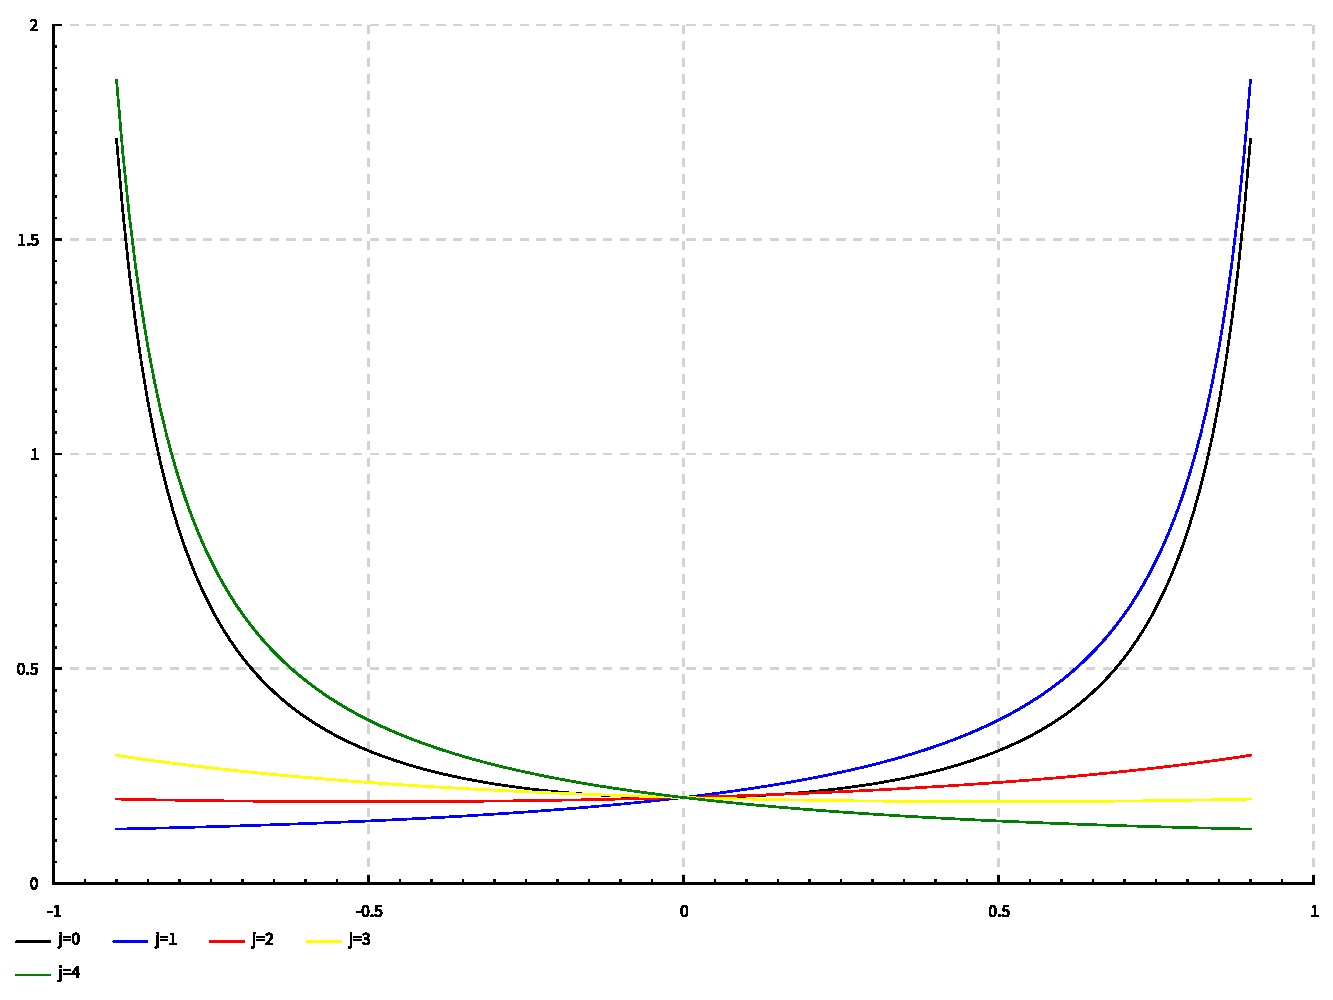
\includegraphics[width=350pt]{images/pi_j}
    \caption{$ f_j(\delta) = \Pi_j(\delta) $}
    \label{fig:pi_j}
\end{figure}

\begin{figure}[htb]
    \centering
    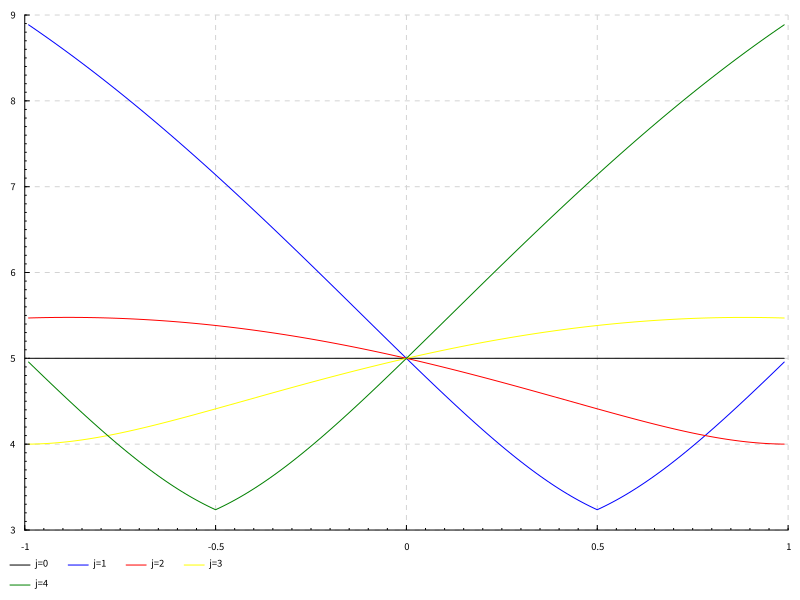
\includegraphics[width=350pt]{images/sigma_row_sum}
    \caption{$ g_j(\delta) = \sum_{r=0}^{n-1} \abs{ \sigma_r^j(z(\delta)) } $}
    \label{fig:sigma_row_sum}
\end{figure}

\begin{figure}[htb]
    \centering
    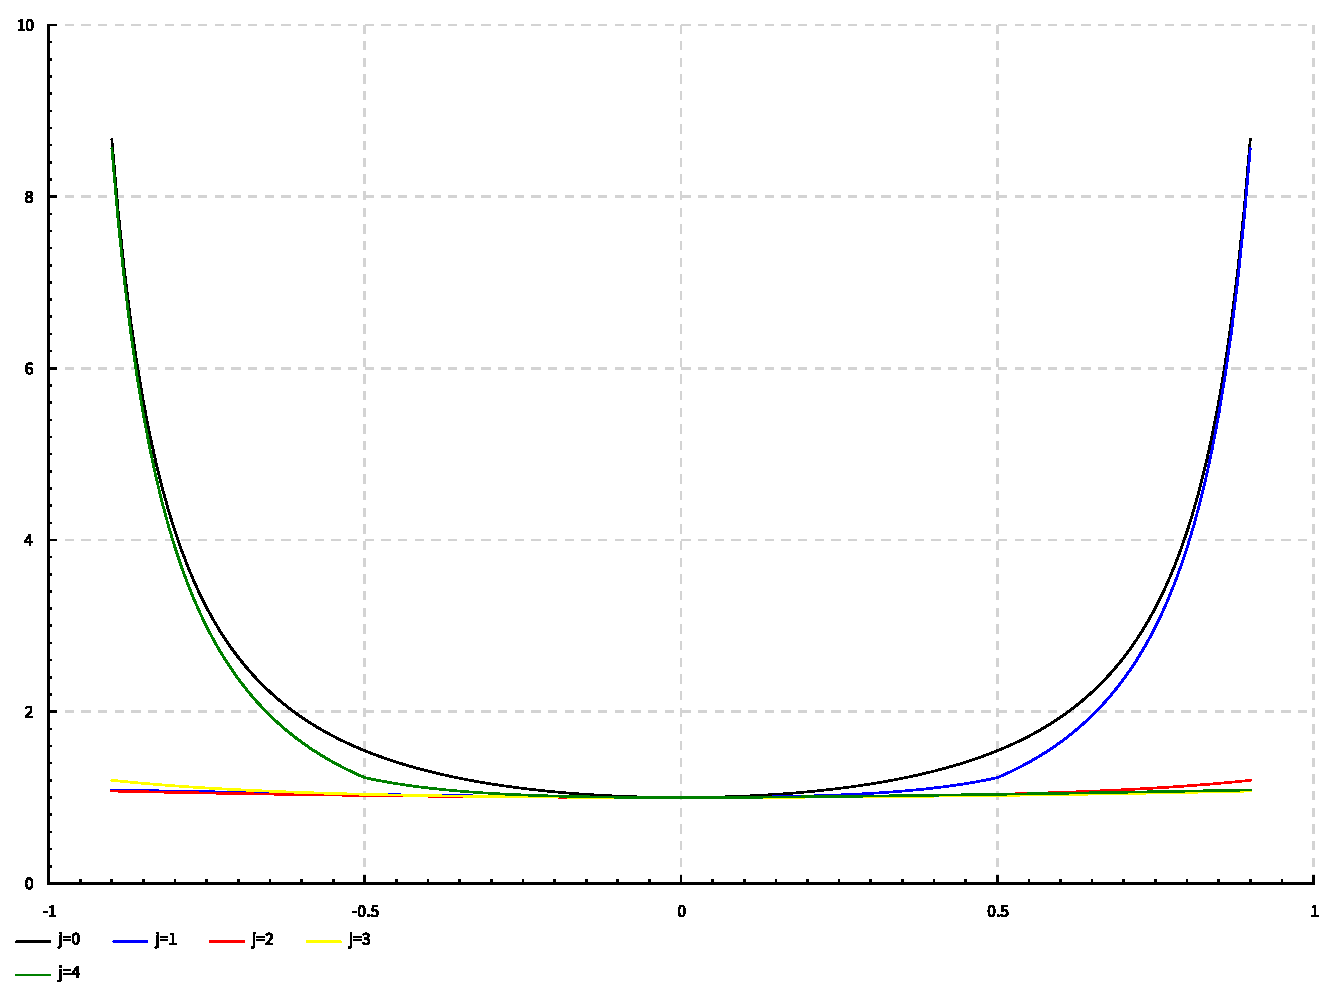
\includegraphics[width=350pt]{images/row_j}
    \caption{$ h_j(\delta) = \sum_{r=0}^{n-1} \abs{ u_{jr}(\delta) } $}
    \label{fig:row_j}
\end{figure}
